\documentclass[oneside,a4paper]{article}

% ========== Preamble (packages, definitions etc.) ==========

\usepackage[utf8]{inputenc}
\usepackage[english]{babel}
\usepackage{graphicx}
\usepackage{xcolor}
\usepackage{amsmath, amsthm, amssymb}
\usepackage{csquotes}
\usepackage{hyperref}
\usepackage{listings}
\usepackage{lmodern}
\usepackage[explicit]{titlesec}
\usepackage{color}
\usepackage{listings}
\lstset{
    breaklines=true,
    basicstyle=\tt\normalsize,
    keywordstyle=\color{blue},
    identifierstyle=\color{magenta},
    frame = single
} 
%\usepackage[backend=bibtex,style=abbrv]{biblatex}
\newcommand{\todo}[1]{{\color{blue}#1}}  % show to-do items in blue
\setlength{\parskip}{\baselineskip}
\usepackage[activate={true,nocompatibility},
            final,
            tracking=true,
            kerning=true,
            %spacing=nonfrench,
            factor=1100,
            stretch=10,
            shrink=10,
            nopatch=eqnum]{microtype}
%\hypersetup{
%    pdftitle={},
%    bookmarks=true,
%    pdfpagemode=FullScreen,
%}

\newcounter{questionnum} \setcounter{questionnum}{0}
%\newcommand{\question}[1]{%
%  \refstepcounter{questionnum}%
%  \paragraph{Question~\arabic{questionnum}:}{\emph{#1}}}

\newcommand\filltoend{\leavevmode{\unskip
  \leaders\hrule height.5ex depth\dimexpr-.5ex+0.4pt\hfill\hbox{}%
  \parfillskip=0pt\endgraf}}

\newcommand{\problem}[2]{%
	\vspace{-0.7em}
	\hspace{0.02\textwidth}
	\begin{minipage}[t][][b]{0.95\textwidth}
		{\bf \hspace{-0.015\textwidth}\makebox[7.5em][l]{{#1} ~~\filltoend}}%
		\hspace{1.2mm}{\it #2}%
	\end{minipage}
}

\definecolor{redbg}{RGB}{235, 214, 214}
\definecolor{Red}{RGB}{163, 25, 25}
\definecolor{Black}{RGB}{0, 0, 0}


\titleformat{\section}
  {\normalfont\LARGE\bfseries}
  {}
  {0em}
  {\colorbox{redbg}{\parbox{\dimexpr\textwidth-2\fboxsep\relax}{\textcolor{Red}{\thesection\quad#1}}}}

\titleformat{\subsection}
  {\normalfont\large\bfseries\color{Black}}
  {\thesubsection}
  {1em}
  {#1}
  [{\titlerule[0.8pt]}]

\titlespacing\subsection{0pt}{12pt plus 4pt minus 2pt}{0pt plus 2pt minus 2pt}

\def\email#1{{\tt#1}}

\lstset{ % Set the default style for code listings
	numbers=left,
	numberstyle=\scriptsize,
	numbersep=8pt,
	basicstyle=\scriptsize\ttfamily,
	keywordstyle=\color{blue},
	stringstyle=\color{red},
	commentstyle=\color{green!70!black},
	breaklines=true,
	frame=single,
	language=bash,
	tabsize=4,
	showstringspaces=false
}
\usepackage{svg}
\usepackage{float}
\usepackage[margin=2cm]{geometry}
\usepackage{pdfpages}
\usepackage[title]{appendix}
\usepackage{indentfirst}
\usepackage{caption, subcaption}
\usepackage{enumitem}


% ========== Title page ==========

\title{
	
\includegraphics[width=0.6\textwidth]{UU_logo.pdf}\\[1em]
	Computer-Assisted Image Analysis I - 1TD396\\[1em]
	Computer Exercise 2\\[3em]
}

\author{
	Jyong-Jhih Lin, \and Linus Falk, \and Niklas Kostrzewa, \and Teng-Sung Yu
	%
}

\date{November 14, 2022}

\begin{document}

\maketitle
\thispagestyle{empty} % Removes page number for front page
\pagebreak

% ========== Document contents ==========
\section{Convolution}
\noindent Use the function conv2 or imfilter to apply different convolution operators to an image. Using the function fspecial you may create different filter kernels to be used. Using the option ’same’ in conv2 you get a result that has the same size as the first argument of the function (typically your image). The commands conv2 and imfilter are similar, but to use conv2 you need to convert the image and the kernel to double before. The imfilter command can filter uint8 images directly.


\subsection*{Q1}
\noindent \textbf{Examine at least 3 different filter kernels, among which there should be at least one sharpening (edge enhancing) and one smoothing filter and apply them in different sizes to the image cameraman.png, e.g. sizes 3 × 3, 7 × 7 and 31 × 31. Note that some filters are only available in one size when using fspecial. Include at least three figures in your report. One showing the original image, one figure showing the image after sharpening, and one figure showing the image after smoothing. For each filter, explain what the filter does to the image, and explain the effect of the different filter sizes.}

The averaging filter replaces the pixel value with the mean value of the neighbor pixels. The selection of neighbors are chosen with the size of the filter kernel. The convolution "drags" this filter kernel through the image and \textbf{smooths} out high frequency changes by averaging the pixel values. The effect of a larger filter kernel is more smoothing as more pixels are included and avereged. Example if this can be see in \ref{fig:Q1a}. 

The Laplacian filter uses the discrete approximation of the second-order derivative. By using this filter we pick up the edges of where the image have changes in intensity, the higher the change the higher the derivative. This result in an image with high pixel intensity values at the places were we have boundaries in the images (often between background and an object). By adding the the filtered image with the high intensities at the boundaries with the original image, we get a result that looks  \textbf{sharper}. 

\begin{figure}[ht!]
\centering
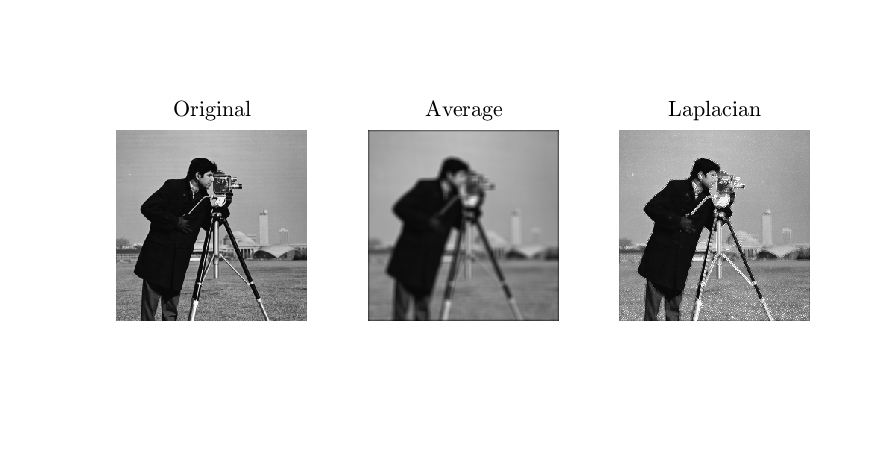
\includegraphics[width=130mm]{figures/Q1b.png}
\caption{Original image and filtered: "Average" and "Laplacian"}
\label{fig:Q1b}
\end{figure}

\begin{figure}[ht!]
\centering
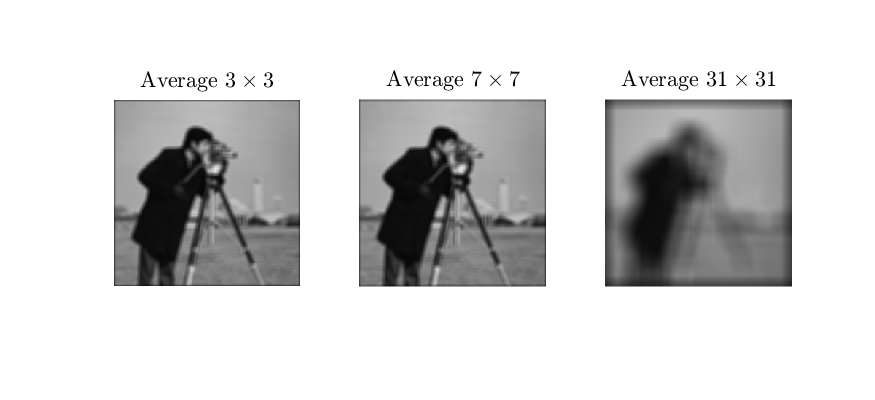
\includegraphics[width=130mm]{figures/Q1a.png}
\caption{"Average" filter of different sizes}
\label{fig:Q1a}
\end{figure}

\newpage

\begin{lstlisting}[language=MATLAB]
laplace_filter = fspecial("laplacian", 0);
mean_filter1 = fspecial("average",3);
mean_filter2 = fspecial("average",7);
mean_filter3 = fspecial("average",31);
disk_filter = fspecial("disk",5);
gauss_filter = fspecial("gaussian");

I = imread("images_lab2/cameraman.png");
Id = double(I);

Imean1 = conv2(Id, mean_filter1, 'same');
Imean1 = uint8(Imean); 

Imean2 = conv2(Id, mean_filter2, 'same');
Imean2 = uint8(Imean2); 

Imean3 = conv2(Id, mean_filter3, 'same');
Imean3 = uint8(Imean3); 

Ilap = conv2(Id,laplace_filter, 'same');
Ilap = uint8(Ilap);

Idisk = conv2(Id, disk_filter, 'same');
Idisk = uint8(Idisk); 

I = imread("images_lab2/cameraman.png");
Id = double(I);

figure(1)
subplot(1,3,1)
imshow(I)
title('Original','Interpreter','latex', 'fontsize',22)
subplot(1,3,2)
imshow(Imean2)
title('Average','Interpreter','latex', 'fontsize',22)
subplot(1,3,3)
imshow(Ilap+I)
title('Laplacian','Interpreter','latex', 'fontsize',22)

figure(2)
subplot(1,3,1)
imshow(Imean2)
title('Average $3\times 3$','Interpreter','latex', 'fontsize',22)
subplot(1,3,2)
imshow(Imean2)
title('Average $7\times 7$','Interpreter','latex', 'fontsize',22)
subplot(1,3,3)
imshow(Imean3)
title('Average $31\times 31$','Interpreter','latex', 'fontsize',22)
\end{lstlisting}

\subsection*{Q2}
\noindent \textbf{Are the filters with filter kernels ’average’, disk’ and gaussian’ examples of low-pass, band-pass or high-pass filters?}

Average, disk and Gaussian are examples of low pass filter. By averaging we smooth out high frequency changes in the image. The Gaussian filter works in a similar way but instead of weighting all neighbors the same, the Gaussian uses the bell-curve/normal distribution curve. The area under the curve is 1 and we get a filter that smooths out rapid changes in intensity, low pass filtering. 
The disk filter is the same as the averaging filter but with a different shape of the kernel, it works like a low pass filter. 

\subsection*{Q3}
\noindent \textbf{Demonstrate how you can synthesize low-pass, band-pass and high-pass filtered images using simple arithmetics and filter kernels mentioned in Question 2.}

\begin{figure}[ht!]
\centering
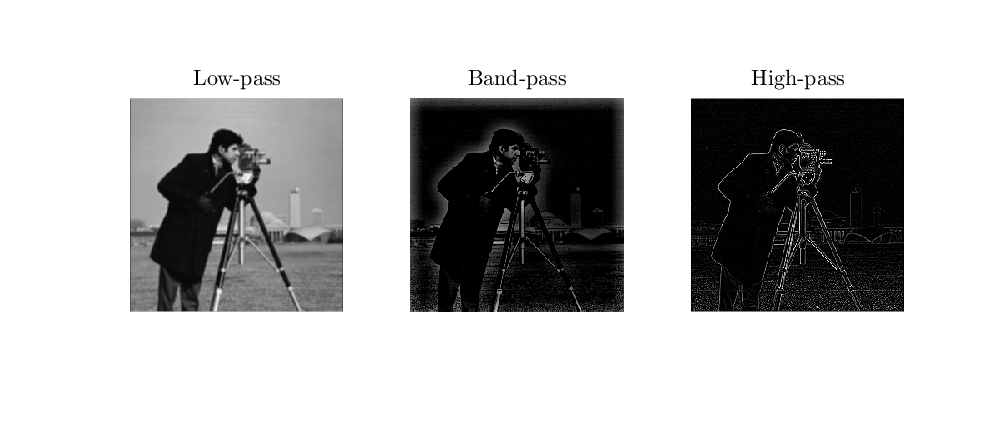
\includegraphics[width=130mm]{figures/Q3.png}
\caption{}
\label{fig:Q3}
\end{figure}

\begin{lstlisting}[language=MATLAB]
laplace_filter = fspecial("laplacian", 0);
mean_filter1 = fspecial("average",3);
mean_filter2 = fspecial("average",7);
mean_filter3 = fspecial("average",31);
disk_filter = fspecial("disk",5);
gauss_filter = fspecial("gaussian");

I = imread("images_lab2/cameraman.png");
Id = double(I);

Imean3 = conv2(Id, mean_filter3, 'same');
Imean3 = uint8(Imean3); 

Ilap = conv2(Id,laplace_filter, 'same');
Ilap = uint8(Ilap);

figure(123)
subplot(1,3,1)
imshow(Imean1)
title('Low-pass','Interpreter','latex', 'fontsize',22)
subplot(1,3,2)
imshow(I-Imean3-Ilap)
title('Band-pass','Interpreter','latex', 'fontsize',22)
subplot(1,3,3)
imshow(Ilap)
title('High-pass','Interpreter','latex', 'fontsize',22)

\end{lstlisting}


\newpage

\section{Sobel filter}
The Matlab function fspecial can produce filter kernels for Sobel filters.
\subsection*{Q4}
\noindent \textbf{Use this functionality to demonstrate Sobel filtering on cameraman.png and wagon.png.
}

\begin{figure}[ht!]
\centering
\includegraphics[width=130mm]{figures/Q4_4_direction_sobel.png}
\caption{Sobel filter}
\label{fig:Q4}
\end{figure}

\begin{lstlisting}[language=MATLAB]
I_cameraman = imread("cameraman.png");
I_wagon = imread("wagon.png");

sobel_filter = fspecial("sobel");

Isobel_l = conv2(I_cameraman, -sobel_filter, 'same');
Isobel_l = uint8(Isobel_l);
Isobel_r = conv2(I_cameraman, sobel_filter, 'same');
Isobel_r = uint8(Isobel_r);
Isobel_u = conv2(I_cameraman, (sobel_filter)', 'same');
Isobel_u = uint8(Isobel_u);
Isobel_d = conv2(I_cameraman, -(sobel_filter)', 'same');
Isobel_d = uint8(Isobel_d);
 
wagon_l = conv2(I_wagon, -sobel_filter, 'same');
wagon_l = uint8(wagon_l);
wagon_r = conv2(I_wagon, sobel_filter, 'same');
wagon_r = uint8(wagon_r);
wagon_u = conv2(I_wagon, (sobel_filter), 'same');
wagon_u = uint8(wagon_u);
wagon_d = conv2(I_wagon, -(sobel_filter)', 'same');
wagon_d = uint8(wagon_d);

figure(4)
subplot(2,2,1)
imshow(Isobel_l+ Isobel_r + Isobel_u + Isobel_d);
title('Sobel filter')
subplot(2,2,2)
imshow(I_cameraman);
title('origin');
subplot(2,2,3)
imshow(wagon_l + wagon_r + wagon_u + wagon_d);
title('Sobel filter')
subplot(2,2,4)
imshow(I_wagon);
title('origin');
\end{lstlisting}



\section{Median filter}
\noindent Median filter is not included in fspecial function and to calculate this filter you can use function medfilt2.


\subsection*{Q5}
\noindent \textbf{Open the image wagon shot noise.png. Perform median filtering on the image using different sizes of the filter masks.}
\begin{lstlisting}[language=MATLAB]
im_wagon_shot = imread('wagon_shot_noise.png');

im_median_filter1 = medfilt2(im_wagon_shot, [3 3]);
im_median_filter2 = medfilt2(im_wagon_shot, [7 7]);


figure(2)
subplot(1,2,1);
imshow(im_median_filter1);
title('filter size 3x3');
subplot(1,2,2);
imshow(im_median_filter2);
title('filter size 7x7');
\end{lstlisting}

\begin{figure}[ht!]
\centering
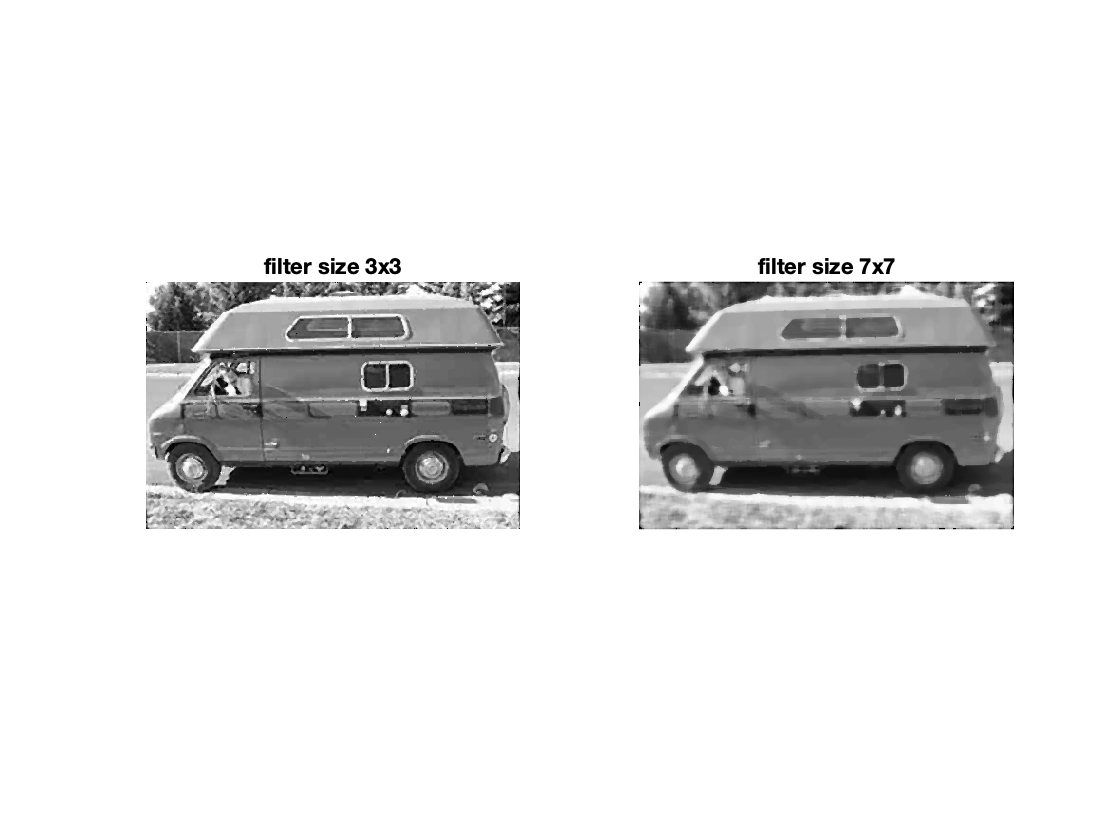
\includegraphics[width=130mm]{figures/Q5.png}
\caption{image of different size of filter}
\label{fig:Q5}
\end{figure}

\subsection*{Q6}
\noindent \textbf{Compare visually the effect of median filtering to the effect of mean and Gauss filtering. Explain the differences on the image wagon shot noise.png. How does median filtering work compare to mean and Gauss filtering?} \\

Median filter work great for pepper salt noise. The median filter replaces the pixel with the median value of the filter window. It works good when the noise is very high or low valued. It also conserves edges better that the other mentioned filters smooths out. The Gaussian average filter works by calculating the new pixel from the whole filter kernel.


\subsection*{Q7}
\noindent \textbf{In general, the median filter is more time consuming, why?}

Matrix multiplication is fast with other filters. Median filter must use some sort of sorting algorithm 

\subsection*{Q8}
\noindent \textbf{Implement your own code for 3x3 median filtering. You may use the Matlab function median that computes the median element of a vector. Use for instance two nested for- loops to iterate your filter for every neighbourhood in the image. The exact behaviour on the borders is not so important for this exercise and you may cut some corners here if it helps you.}
\begin{lstlisting}[language=MATLAB]
result = zeros(260,394);
Jr = I_wagon_noise;
for i=2:259
    for j = 2:393
        result(i,j) = median(Jr((i-1):(i+1),(j-1):(j+1)),'all');   
    end
end

result = uint8(result);

figure(4)
subplot(1,2,1)
imshow(I_wagon_noise)
subplot(1,2,2)
imshow(result)

\end{lstlisting}

\subsection*{Q9}
\noindent \textbf{If you implement a Gaussian filter using a large filter mask (and a large standard deviation), why do you get a black border around the image?}

This is probably caused by the padding method set "zero method" in which we pad the image with zeros around the edges to have values for our filter to average over.  

\newpage

\section{Fast Fourier Transform }
\noindent Open the image lines.png. Transform the image using the FFT and display the logarithm of the magnitude of the Fourier components. Can you see a relationship between the lines in the Fourier spectra and the lines in the original image? 


\subsection*{Q10}
\noindent \textbf{Repeat the same procedure with the image cameraman.png. Comment on the spectrum that you see and compare it to the ordinary representation of the image. You may also try other images, for example circle.png or rectangle.png.}

\noindent Edges show up as "lines/streaks". The vertical line is associated with the horizontal lines in the image, like his shoulder and the buildings in the background. The streak with angle approx 30 deg correspond to the sharp edges in that angle in the image, like the tripod legs. 

\begin{figure}[ht!]
\centering
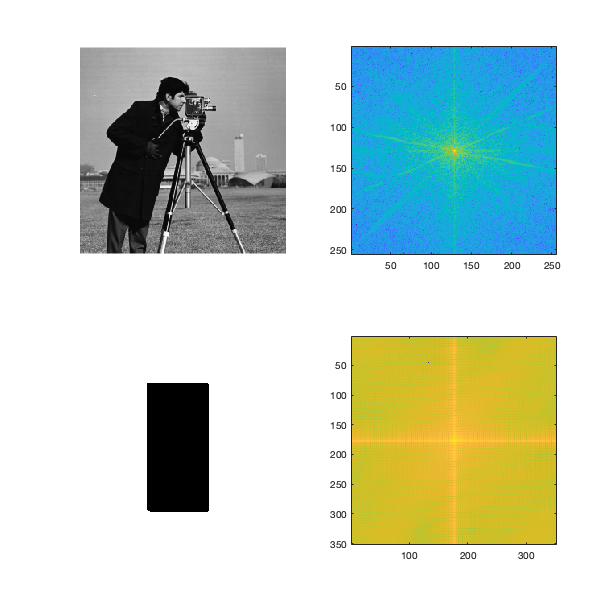
\includegraphics[width=100mm]{figures/Q10.png}
\caption{}
\label{fig:Q10}
\end{figure}

\begin{lstlisting}[language=MATLAB]
I = imread("images_lab2/cameraman.png");
I2 = imread("images_lab2/rectangle.png");


edit = ones(2)-10e6;
edit = padarray(edit, [127, 127]);


im = double(I);
f = fftshift(fft2(im));
im2 = double(I2);
f2 = fftshift(fft2(im2));


subplot(2,2,1);
imshow(uint8(I))
subplot(2,2,2);
imagesc(log(abs(f)));
subplot(2,2,3);
imshow(uint8(I2))
subplot(2,2,4);
imagesc(log(abs(f2)));

figure(3)
f3 = fftshift(fft2(rand(1,5)));
imagesc(log(abs(f3))); 
\end{lstlisting}


\subsection*{Q11}
\noindent \textbf{Experiment with FFT of an odd-length signal (image) of small length. For creating such a signal (image) use the command ... }

For odd length signal the Fourier transform is symmetric and (1,3) is real valued
\begin{equation}
\begin{bmatrix} -0.1082 + 0.9086i&   0.4484 - 0.2022i&   3.3932 + 0.0000i&   0.4484 + 0.2022i&  -0.1082 - 0.9086i \end{bmatrix}
\nonumber
\end{equation}

The symmetry pattern repeated with even length if not including the first element which is real. The first (1,1) and (1,3) is real valued.
\begin{equation}
\begin{bmatrix} -0.8775 + 0.0000i&   0.6877 - 0.0076i&   2.7609 + 0.0000i&   0.6877 + 0.0076i \end{bmatrix}
\nonumber
\end{equation}

Putting only (1,2) to 0 results in a complex valued image after inverse transform. Putting (1,4) to zero makes it real valued. By changing the elements symmetrically we ensure that we receive a real valued image after inverse transformation. 


\subsection*{Q12}
\noindent \textbf{Now modify the FFT representation of cameraman.png, by setting certain frequencies to 0, to create a low-pass version of the image. Use a circular filter for the best result, but feel free to simplify the task with a square pattern of your filter. You may blank out a part of a matrix using slices ...}

\begin{figure}[ht!]
\centering
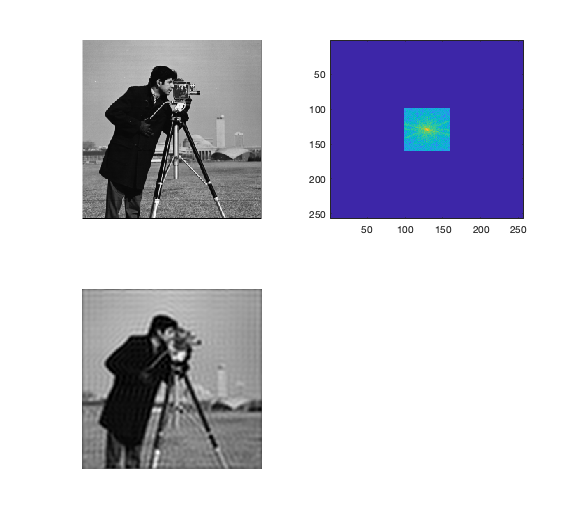
\includegraphics[width=100mm]{figures/Q12.png}
\caption{}
\label{fig:Q12}
\end{figure}

\begin{lstlisting}[language=MATLAB]
I = imread("images_lab2/cameraman.png");
padda = zeros(257);
padda2 = zeros(257);
padda(1:256,1:256) = I;

c = 30;

padda_f = fftshift(fft2(padda));
padda2(129-c:129+c, 129-c:129+c) = padda_f(129-c:129+c, 129-c:129+c);
im = ifft2(ifftshift(padda2));
im = uint8(im);

filtered = im(1:256,1:256);

figure(97)
subplot(2,2,1);
imshow(uint8(padda));
subplot(2,2,2);
imagesc(log(abs(padda2)));
subplot(2,2,3);
imshow(filtered);

\end{lstlisting}


\subsection*{Q13}
\noindent \textbf{Create a filter in the frequency-domain that suppresses the pattern in freqdist.png, but leaves the rest of the image as intact as possible. What does the filter look like? What do you see in the filtered image? Like the previous question, the resulting image should be real-valued after performing ifft. You are not allowed to use the functions real or abs or similar ways to force a real-valued result.}

The filter is a notch filter and looks like four "holes" were it previously were bright dots caused by the periodic "noise" in the image. The image after filtering shows an aerial image over some houses and perhaps a river or a road. 

\begin{figure}[ht!]
\centering
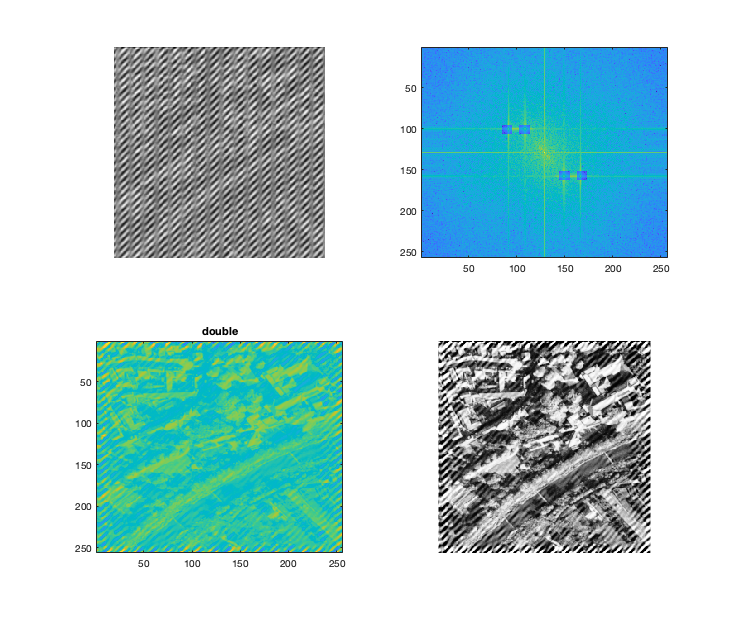
\includegraphics[width=100mm]{figures/Q13.png}
\caption{}
\label{fig:Q13}
\end{figure}

\begin{lstlisting}[language=MATLAB]
I = imread("images_lab2/freqdist.png");

I_p = zeros(257);
I_p(1:256,1:256) = I;
c = 5;

filter = fspecial("gaussian", c*2+1, 5); 
%filter = fftshift(fft2(filter));
I_f = fftshift(fft2(I_p));


 
I_f(101-c:101+c,108-c:108+c) = I_f(101-c:101+c,108-c:108+c) .* filter;
I_f(157-c:157+c,150-c:150+c) = I_f(157-c:157+c,150-c:150+c) .* filter;

I_f(101-c:101+c,90-c:90+c) = I_f(101-c:101+c,90-c:90+c) .* filter;
I_f(157-c:157+c,168-c:168+c) = I_f(157-c:157+c,168-c:168+c) .* filter;



figure(111)
subplot(2,2,1)
imshow(I)
subplot(2,2,2)
imagesc(log(abs(I_f)))
subplot(2,2,3)
im = ifft2(ifftshift(I_f));
filtered = im(1:256,1:256);
imagesc(filtered)
title((class(filtered)))
im = cast(filtered,'uint8');
im = histeq(im);
subplot(2,2,4)
imshow(im)

\end{lstlisting}

% Delete this section if you have no plot to submit.
% Change the size of the figure by changing the value in [width=300pt]

% Putting \autoref{fig:my_figure} in your text will refer to the corresponding figure label.
% Eg.: "\autoref{fig:my_figure} clearly shows that the large circle is larger than the small box."
% Read more about autoref here https://en.wikibooks.org/wiki/LaTeX/Labels_and_Cross-referencing#autoref

%\bibliographystyle{apalike}
%\bibliographystyle{abbrv}
%\bibliography{bibliography}

\end{document}